\documentclass{article}

\usepackage{scribe}
\usepackage{pgfplots}

\setseriestitle{ECO754A: Game Theory}
\setscribecode{8}
\setinstrname{Dr. Vimal Kumar}
\setauthname{Gurpreet Singh}
\setauthemail{guggu@iitk.ac.in}
\settitle{Evolutionary Game Theory}

\begin{document}
\makeheader

\begin{ssection}{Inroduction}

	Classical game theory was developed to model competitions between adversaries which are assumed to be conscious, rational, and in control of their decisions. This has been an implicit assumption in all our discussions so far. However, often this does not hold, such as in evolutionary biology, around which our discussion lies for this lecture. We take a look at an application of game theory in the setting of evolutionary biology (for simple scenarios) where the decisions are inconscious, and often not in the hands of the players at all.

	This application of game theory to evolving populations in biology is termed as \et{Evolutionary Game Theory} \citep{smith}. Evolutionary biology is based on the idea that an organism’s genes largely determine its observable characteristics, and hence its fitness in a given environment. Organisms that are more fit will tend to produce more offspring, causing genes that provide greater fitness to increase their representation in the population. In this way, fitter genes tend to win over time, because they provide higher rates of reproduction \citep{kleinberg}. With game theory, it becomes possible to understand the behaviour of these organisms based on their inherited genetic encoding.

	% Evolutionary game theory also gives the basis to explaining altruistic behaviour as a benefitial strategy for the stability of a species.

\end{ssection}

\begin{ssection}{Interaction and Strategies}

	In biology, strategies are genetically inherited traits that control an individual's action, analogous with computer programs. \citep{wiki}. Evolutionary game theory relies on the interactions among players based on these strategies. In order to explain this, we consider a simple example of a species of beetles with two different sets of \et{phenotypes}, coexisting in the same environment.

	\ditem{The Beetles Game} We consider two phenotypes of beetles, large body beetles and small body beetles. These inherited traits of body size are, therefore, the strategies which are not in control of the players \ie the organisms. The fitness of the beetles is defined by the amount of nutrients it can consume, or the amount of food that is avalaible to it.

	In an ideal scenario, where each beetle is provided the same amount of food, beetles with smaller bodies will have achieved a higher level of fitness due to the lower metabolic requirements. However, due to interaction between the beetles, this scenario does not hold.

	As mentioned, there will be interaction, rather competition, between different phenotypes and the total food will be split into different ratios. The problem of interest here is understanding the evolutionary coexistence of the two phenotypes. We start with defining the properties of these interactions as decided by the environment. There are simple assumptions to this game as given below --
	\begin{enumerate}
		\item Smaller beetle achieves a higher level of fitness assuming same amount of food consumed
		\item Larger beetle is able to procure more food when interacting/competing with a small beetle
		\item The food is equally shared among beetles of the same size
	\end{enumerate}

	We can represent this game using a payoff matrix (refer to table \ref{tab:beetle-payoffs}) which follows the assumptions listed above, The payoff, in this case, is defined to be the level of fitness achieved when two beetles are interacting or dividing a sharable resource of food, assuming the same amount of food to be available in every interaction.

	\begin{table}
		\centering
		\begin{tabular}{c | c | c}
			& \bt{Small} & \bt{Large} \\
			\hline
			\bt{Small} & 6 & 1 \\
			\bt{Large} & 10 & 4 \\
		\end{tabular}
		\caption{Payoff Matrix for Beetles Game}
		\label{tab:beetle-payoffs}
	\end{table}

	The payoff matrix is a way to summarize the properties of all interactions possible in the game. These strategies to be played in such games are hardwired into the genetic encoding of the players, rather than being conscious choices, as the interactions are completely dependent upon the ratio of the population of small versus large beetles. Our interest lies in studying these strategies \ie the existence of each phenotypes in the environment. The notion of Nash Equilibrium does not obviously extend as there is no agent choosing its strategies. Therefore, we define an alternate notion of stability, \et{Evolutionary Stable Strategies}.

\end{ssection}

\begin{ssection}{Evolutionary Stable Strategies}

	Although we do not have an obvious notion of an ``equilibrium'' in this case, we define an analogous stability measure, and any ``stable'' strategy resulting in an equilibrium is known as an \et{Evolutionary Stable Strategies} (ESS).

	The equilibrium, in case of evolutionary biology, is the choice of strategies for each organism such that the coexistence of different organisms is stable, \ie small changes or rather mutations to the existing choice of species eventually return to the same original mix of strategies. This choice of strategies, however, might not be in the hands of the players/organisms, but are inherited traits, as mentioned earlier.

	Before looking at the formal definition of evolutionary stable strategies, we will try to find (by building up intuition) an equilibrium for the beetles game.

	\begin{sssubsection}{The Beetles Game}

		For the beetles game, we have two strategies \et{Small} (represented as S) and \et{Large} (represented as L) for each organism. If we disallow any mixed strategies, we are essentially assuming that the complete population of beetles are using only one of the strategies (large and small). In order to check whether a strategy is an ESS, we introduce small levels of mutation and check whether there is evolution tendency to return back to the original strategy as a check for stability.

		Suppose we consider the strategy S first. We assume that the complete population uses S, and a small mutation of level $\epsilon$ is introduced, \ie a small ratio ($\epsilon$) of the population now uses L. Note that this mutation in induced by an external agent, such as a human in a test lab. The tendency to shift is provided by the different levels of fitness among the organisms using different strategies. As mentioned in the first section, a phenotype/species with a larger level of fitness tends to have a larger rate of reproduction. This determines the future mix of strategies among the population, and therefore decides the stability of a strategy.

		In order to determine the fitness levels, we consider the average fitness of organisms using different strategies. Following the payoff matrix given in table \ref{tab:beetle-payoffs}, we can say that a beetle using the strategy S would achieve a payoff/fitness level of 6 when interacting with a small beetle and payoff of 1 when interacting with a large beetle. Since the ratio of the number of beetles using the strategy S to the total population is $(1 - \eps)$, we can write (using rule of probability) the expected payoff to be $6 \cdot (1 - \eps) + 1 \cdot \eps = 6 - 5\eps$.

		Similarly, for a beetle using L, the average/expected payoff will be $10 \cdot (1 - \eps) + 4 \cdot \eps = 10 - 6 \eps$. Since $\eps$ is a ratio, we have $0 < \eps < 1$. Plotting these two lines (refer to figure \ref{fig:beetle-small-ess}) reveals that the average payoff/fitness of the larger beetles would be higher for any given $0 < \eps < 1$. This suggests that over time, large bodied beetles will take over the population of small bodied beetles. Therefore, we can say that introduction a small level of mutation to the strategy S would cause the coexistence ratio to change and hence,the strategy S is not an evolutionary stable strategy.

		\begin{figure}[htpb]
			\centering
			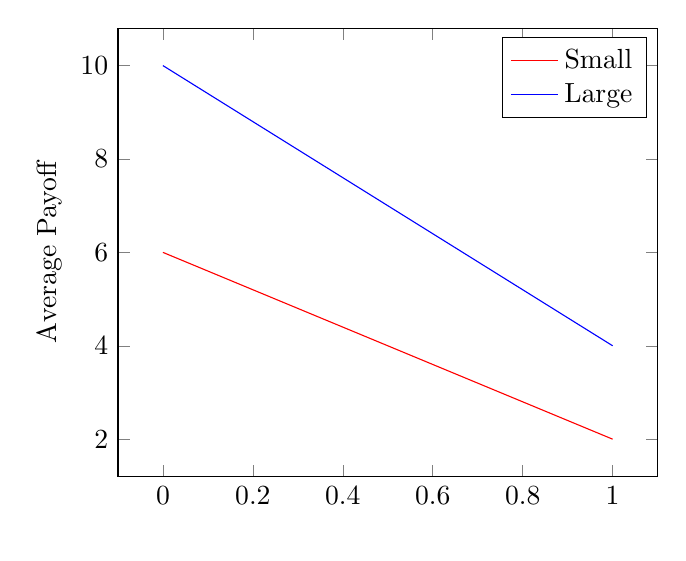
\begin{tikzpicture}
				\begin{axis}[
						xlabel = $\eps$,
						ylabel = Average Payoff,
					]
					\addplot[
						color=red,
						domain=0:1
					]{6 - 4 * x};
					\addlegendentry{Small};
					\addplot[
						color=blue,
						domain=0:1
					]{10 - 6 * x};
					\addlegendentry{Large};
				\end{axis}
			\end{tikzpicture}
			\caption{Plot of Average Payoffs vs level of mutation}
			\label{fig:beetle-small-ess}
		\end{figure}

		If we assume the whole population to be of large beetles, and introduce a small level of mutation via adding small beetles, we can do the same calculations to verify that the average payoffs for large beetles will be higher for any level of mutation. This can be also be understood as replacing $\eps$ with $1 - \eps$ in figure \ref{fig:beetle-small-ess}. Therefore, we can conclude that the strategy L is an ESS whereas strategy S is not an ESS, or equivalently, large beetles are evolutionary stable whereas small beetles are not.

	\end{sssubsection}

	We formally define the introduction of mutation (as used above) as the invasion of one strategy by another. We say that a strategy T invades a strategy S at level $\eps$, for some small positive number $\eps$, if an $\eps$ fraction of the underlying population uses T and a $1 - \eps$ fraction of the underlying population uses S. Using this and the intuition built from the example of the Beetles game, we can now formally define an Evolutionary Stable Strategy following the example discussed above.

	\begin{definition}[Evolutionary Stable Strategy]
		We say that a strategy S is an \et{Evolutionary Stable Strategy} (ESS) iff there is a (small) positive number $y$ such that when any other strategy T invades S at any level $0 < x < y$, the fitness (average payoff) of an organism playing S is strictly greater than the fitness of an organism playing T.
		\label{def:ess}
	\end{definition}

	In the beetles game, we found the small body beetles to be evolutionary unstable. This means that a small population of large beetles introduced into a pure population of small beetles have higher average fitness than the small beetles, and therefore persist in the environment. On the other hand, a small population of small beetles introduced into a pure population of large beetles will be driven out, and therefore the large body beetles are evolutionary stable.

\end{ssection}

\begin{ssection}{The Hawk-Dove Game}

	The classic Hawk Dove game (a derivative of the Chicken game) was the first game that was analysed using Evolutionary Game Theory by \cite{smith}. The Hawk Dove game defines a contest over sharable resources divided amongst a population of Doves and/or Hawks. These are two phenotypes of the same species.

	The fitness (payoff) assumptions of the game are as follows
	\begin{enumerate}
		\item If a Hawk meets a Dove he gets the full resource to himself -- V
		\item If a Hawk meets a Hawk, there is a conflict and both the birds are injured -- V/2 - C/2 (C $\gg$ V).
		\item If a Dove meets a Hawk he chickens out, and therefore gets nothing -- 0
		\item If a Dove meets a Dove both share the resource -- V/2
	\end{enumerate}

	We represent this in a payoff matrix as given in table \ref{tab:payoff-dhg}.

	\begin{table}
		\centering
		\begin{tabular}{c | c | c}
			& \bt{Hawk} & \bt{Dove} \\
			\hline
			\bt{Hawk} & V/2 - C/2 & V \\
			\hline
			\bt{Dove} & 0 & V/2
		\end{tabular}
		\caption{Payoff Matrix for the Dove Hawk game}
		\label{tab:payoff-dhg}
	\end{table}

	\bt{Finding the Evolutionary Stable Strategies.} \ \ We first check whether Doves are evolutionary stable or not. In order to do this, we introduce a small population (say $\eps$) of Doves. Therefore the ratio of populations of Doves to Hawks is $\eps / (1 - \eps)$. We can now write the average fitness for hawks and doves. Similar to the Beetles game, with probability $1 - \eps$ the interaction is with a dove, and with probability $\eps$ the interaction is with a hawk. Therefore the average fitness of doves ($f_D$) and hawks ($f_H$) are given as
	\begin{align*}
		f_D &\eq \sV/2 \cdot (1 - \eps) + 0 \cdot \eps \\&\eq \frac{1}{2} \sV \cdot (1 - \eps) \\
		f_H &\eq \sV \cdot (1 - \eps) + \para{\sV/2 - \sC/2} \cdot \eps \\&\eq \sV - \frac{1}{2} (\sV + \sC) \cdot \eps
	\end{align*}

	Clearly, as $\eps \ra 0$, $f_H > f_D$. Therefore, doves are not evolutionary stable in the Dove Hawk Game. We can do the same analysis for hawks as well. In this case, we assume an invasion of doves at level $\eps$ to a population of hawks. Therefore the average fitness gained can be written as
	\begin{align*}
		f_D &\eq 0 \cdot (1 - \eps) + \sV/2 \cdot \eps \\ &\eq \frac{1}{2} \sV \cdot (1 - \eps) \\
		f_H &\eq (\sV/2 - \sC/2) \cdot (1 - \eps) + \sV \cdot \eps \\ &\eq \frac{1}{2} \para{\sV - \sC +(\sV + \sC) \cdot \eps}
	\end{align*}

	In this case, as $\eps \ra 0$, we have $f_H < f_D$. Therefore, hawks aren't evolutionary stable either.

\end{ssection}

\begin{ssection}{Relation with Nash Equilibrium}

	Suppose we have two strategies A and B in a symmetric game, such as the Beetles game and the Dove Hawk game. We can formulate them in the form of a tabular game as given in table \ref{tab:gen-game}.

	\begin{table}
		\centering
		\begin{tabular}{c c c c}
			& & \multicolumn{2}{c}{Player 2} \\
			& & \bt{A} & \bt{B} \\
			\cline{3-4}
			\multirow{2}{*}{Player 1} & \bt{A} & \multicolumn{1}{|c}{a, a} & \multicolumn{1}{|c|}{b, c} \\
			\cline{3-4}
			& \bt{B} & \multicolumn{1}{|c}{c, b} & \multicolumn{1}{|c|}{d, d} \\
			\cline{3-4}
		\end{tabular}
		\caption{General Symmetric Game}
		\label{tab:gen-game}
	\end{table}

	If we say that the B is invading A at a level $\eps$, then the expected payoff to an organism playing A in a random interaction is given as \[f_A = a \cdot (1 - \eps) + b \cdot \eps\]
	In the same case, the expected payoff to an organism playing B is \[f_B = c \cdot (1 - \eps) + d \cdot \eps\]

	In order to claim that A is evolutionary stable, we need to have the expected payoff of an organism playing A to be strictly greater than an organism playing B. Therefore, we have
	\begin{align*}
		a \cdot (1 - \eps) + b \cdot \eps \qgt c \cdot (1 - \eps) + d \cdot \eps
	\end{align*}

	In case $a > c$, we have $f_A > f_B$ for small enough $\eps$. Therefore in this case, A is an ESS. In case $a < c$, we have $f_A < f_B$ for $\eps \ra 0$, therefore A is not an ESS. Suppose if $a = c$, then we need to have $b > d$ such that $f_A > f_B$.

	We can formalize this by saying if A is an ESS, then we need to have
	\begin{align*}
		(i) \ a > c \quad \text{or} \quad (ii) \ a = c \ \mt{ and } b > d
	\end{align*}

	In either case, we have $a \ge c$, which is sufficient and necessary for the (A, A) to be a Nash Equilibrium. Therefore, we can say that if A is an ESS, then (A, A) is a Nash Equilibrium.

	We will take a deeper look at this relation in the next lecture. We will also discuss the notion of evolutionary stable strategies in games with more than two strategies, and with mixed strategies as well.

\end{ssection}

\bibliographystyle{plainnat}
\bibliography{references}

\end{document}
